% Options for packages loaded elsewhere
\PassOptionsToPackage{unicode}{hyperref}
\PassOptionsToPackage{hyphens}{url}
%
\documentclass[
  letterpaper,
]{scrbook}

\usepackage{amsmath,amssymb}
\usepackage{iftex}
\ifPDFTeX
  \usepackage[T1]{fontenc}
  \usepackage[utf8]{inputenc}
  \usepackage{textcomp} % provide euro and other symbols
\else % if luatex or xetex
  \usepackage{unicode-math}
  \defaultfontfeatures{Scale=MatchLowercase}
  \defaultfontfeatures[\rmfamily]{Ligatures=TeX,Scale=1}
\fi
\usepackage{lmodern}
\ifPDFTeX\else  
    % xetex/luatex font selection
\fi
% Use upquote if available, for straight quotes in verbatim environments
\IfFileExists{upquote.sty}{\usepackage{upquote}}{}
\IfFileExists{microtype.sty}{% use microtype if available
  \usepackage[]{microtype}
  \UseMicrotypeSet[protrusion]{basicmath} % disable protrusion for tt fonts
}{}
\makeatletter
\@ifundefined{KOMAClassName}{% if non-KOMA class
  \IfFileExists{parskip.sty}{%
    \usepackage{parskip}
  }{% else
    \setlength{\parindent}{0pt}
    \setlength{\parskip}{6pt plus 2pt minus 1pt}}
}{% if KOMA class
  \KOMAoptions{parskip=half}}
\makeatother
\usepackage{xcolor}
\setlength{\emergencystretch}{3em} % prevent overfull lines
\setcounter{secnumdepth}{5}
% Make \paragraph and \subparagraph free-standing
\ifx\paragraph\undefined\else
  \let\oldparagraph\paragraph
  \renewcommand{\paragraph}[1]{\oldparagraph{#1}\mbox{}}
\fi
\ifx\subparagraph\undefined\else
  \let\oldsubparagraph\subparagraph
  \renewcommand{\subparagraph}[1]{\oldsubparagraph{#1}\mbox{}}
\fi


\providecommand{\tightlist}{%
  \setlength{\itemsep}{0pt}\setlength{\parskip}{0pt}}\usepackage{longtable,booktabs,array}
\usepackage{calc} % for calculating minipage widths
% Correct order of tables after \paragraph or \subparagraph
\usepackage{etoolbox}
\makeatletter
\patchcmd\longtable{\par}{\if@noskipsec\mbox{}\fi\par}{}{}
\makeatother
% Allow footnotes in longtable head/foot
\IfFileExists{footnotehyper.sty}{\usepackage{footnotehyper}}{\usepackage{footnote}}
\makesavenoteenv{longtable}
\usepackage{graphicx}
\makeatletter
\def\maxwidth{\ifdim\Gin@nat@width>\linewidth\linewidth\else\Gin@nat@width\fi}
\def\maxheight{\ifdim\Gin@nat@height>\textheight\textheight\else\Gin@nat@height\fi}
\makeatother
% Scale images if necessary, so that they will not overflow the page
% margins by default, and it is still possible to overwrite the defaults
% using explicit options in \includegraphics[width, height, ...]{}
\setkeys{Gin}{width=\maxwidth,height=\maxheight,keepaspectratio}
% Set default figure placement to htbp
\makeatletter
\def\fps@figure{htbp}
\makeatother

\makeatletter
\@ifpackageloaded{tcolorbox}{}{\usepackage[skins,breakable]{tcolorbox}}
\@ifpackageloaded{fontawesome5}{}{\usepackage{fontawesome5}}
\definecolor{quarto-callout-color}{HTML}{909090}
\definecolor{quarto-callout-note-color}{HTML}{0758E5}
\definecolor{quarto-callout-important-color}{HTML}{CC1914}
\definecolor{quarto-callout-warning-color}{HTML}{EB9113}
\definecolor{quarto-callout-tip-color}{HTML}{00A047}
\definecolor{quarto-callout-caution-color}{HTML}{FC5300}
\definecolor{quarto-callout-color-frame}{HTML}{acacac}
\definecolor{quarto-callout-note-color-frame}{HTML}{4582ec}
\definecolor{quarto-callout-important-color-frame}{HTML}{d9534f}
\definecolor{quarto-callout-warning-color-frame}{HTML}{f0ad4e}
\definecolor{quarto-callout-tip-color-frame}{HTML}{02b875}
\definecolor{quarto-callout-caution-color-frame}{HTML}{fd7e14}
\makeatother
\makeatletter
\makeatother
\makeatletter
\@ifpackageloaded{bookmark}{}{\usepackage{bookmark}}
\makeatother
\makeatletter
\@ifpackageloaded{caption}{}{\usepackage{caption}}
\AtBeginDocument{%
\ifdefined\contentsname
  \renewcommand*\contentsname{Table of contents}
\else
  \newcommand\contentsname{Table of contents}
\fi
\ifdefined\listfigurename
  \renewcommand*\listfigurename{List of Figures}
\else
  \newcommand\listfigurename{List of Figures}
\fi
\ifdefined\listtablename
  \renewcommand*\listtablename{List of Tables}
\else
  \newcommand\listtablename{List of Tables}
\fi
\ifdefined\figurename
  \renewcommand*\figurename{Figure}
\else
  \newcommand\figurename{Figure}
\fi
\ifdefined\tablename
  \renewcommand*\tablename{Table}
\else
  \newcommand\tablename{Table}
\fi
}
\@ifpackageloaded{float}{}{\usepackage{float}}
\floatstyle{ruled}
\@ifundefined{c@chapter}{\newfloat{codelisting}{h}{lop}}{\newfloat{codelisting}{h}{lop}[chapter]}
\floatname{codelisting}{Listing}
\newcommand*\listoflistings{\listof{codelisting}{List of Listings}}
\makeatother
\makeatletter
\@ifpackageloaded{caption}{}{\usepackage{caption}}
\@ifpackageloaded{subcaption}{}{\usepackage{subcaption}}
\makeatother
\makeatletter
\@ifpackageloaded{tcolorbox}{}{\usepackage[skins,breakable]{tcolorbox}}
\makeatother
\makeatletter
\@ifundefined{shadecolor}{\definecolor{shadecolor}{rgb}{.97, .97, .97}}
\makeatother
\makeatletter
\makeatother
\makeatletter
\makeatother
\ifLuaTeX
  \usepackage{selnolig}  % disable illegal ligatures
\fi
\IfFileExists{bookmark.sty}{\usepackage{bookmark}}{\usepackage{hyperref}}
\IfFileExists{xurl.sty}{\usepackage{xurl}}{} % add URL line breaks if available
\urlstyle{same} % disable monospaced font for URLs
\hypersetup{
  pdftitle={Digital urban in workshop},
  hidelinks,
  pdfcreator={LaTeX via pandoc}}

\title{Digital urban in workshop}
\author{}
\date{}

\begin{document}
\frontmatter
\maketitle
\ifdefined\Shaded\renewenvironment{Shaded}{\begin{tcolorbox}[interior hidden, borderline west={3pt}{0pt}{shadecolor}, boxrule=0pt, frame hidden, enhanced, sharp corners, breakable]}{\end{tcolorbox}}\fi

\renewcommand*\contentsname{Table of contents}
{
\setcounter{tocdepth}{2}
\tableofcontents
}
\mainmatter
\bookmarksetup{startatroot}

\hypertarget{welcome}{%
\chapter*{Welcome}\label{welcome}}
\addcontentsline{toc}{chapter}{Welcome}

\markboth{Welcome}{Welcome}

Andy MacLachlan\footnote{The Bartlett Centre for Advanced Spatial
  Analysis, https://twitter.com/andymaclachlan}

Last updated: \texttt{r\ Sys.Date()}

Hello and welcome to the Term 2 module Remotely Sensing Cities and
Environments.

This website holds the material used to support work the Critical
interrogations of the digital urban in India workshop that is being held
here at the Indian Institute of Technology Hyderabad on 19 July 2023.

\bookmarksetup{startatroot}

\hypertarget{software-installation}{%
\chapter*{Software installation}\label{software-installation}}
\addcontentsline{toc}{chapter}{Software installation}

\markboth{Software installation}{Software installation}

This course primarily uses the R data science programming language. We
briefly touch upon QGIS to give you a basic foundation in the range of
spatial software available, please follow the instructions below before
the first practical session to install the software on your local
computer if you are planning to use it throughout the course.

\hypertarget{qgis}{%
\section*{QGIS}\label{qgis}}
\addcontentsline{toc}{section}{QGIS}

\markright{QGIS}

QGIS is an open-source graphic user interface GIS with many community
developed add on packages that (or plugins) that provide additional
functionality to the software.

To get QGIS on your personal machine go to:
https://qgis.org/en/site/forusers/download.html

I install the OSGeo4W version. The nature of open-source means that
several programs will rely on each other for features. OSGeo4W tracks
all the shared requirements and does not install any duplicates.

When you click through the dialogue boxes you need to \textbf{search for
QGIS in the OSGeo4W setup and click the refresh button} so it
\textbf{changes from skip to install}\ldots.

\begin{figure}

{\centering 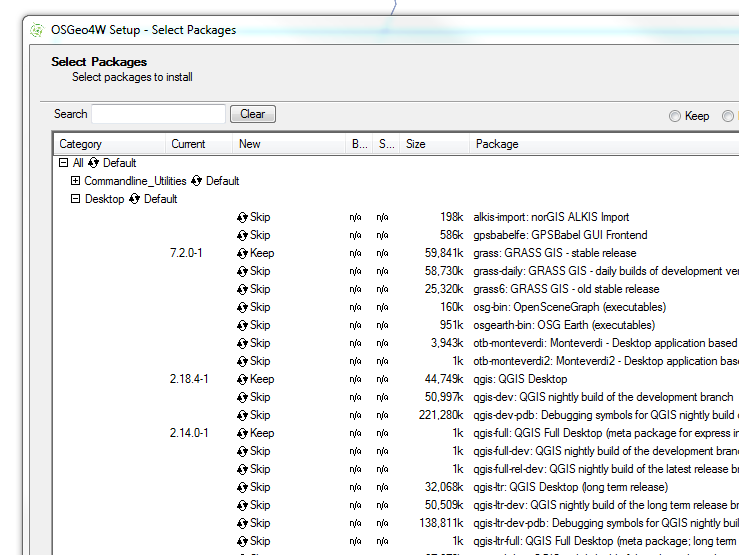
\includegraphics[width=4.6875in,height=\textheight]{general_images/QGIS_install2.png}

}

\caption{Continuous and discrete data. Source:
\href{https://gis.stackexchange.com/questions/230672/how-to-install-osgeo4w-libraries-in-older-version-of-qgis-2-16}{GIS
Stackexchange}}

\end{figure}

\bookmarksetup{startatroot}

\hypertarget{spatial-data}{%
\chapter{Spatial data}\label{spatial-data}}

\hypertarget{spatial-data-1}{%
\section{Spatial data}\label{spatial-data-1}}

Geographic data, geospatial data or geographic information is data that
identifies the location of features on Earth. There are two main types
of data which are used in GIS applications to represent the real world.

\begin{itemize}
\item
  Vectors that are composed of points, lines and polygons
\item
  Rasters that are grids of cells with individual values\ldots{}
\end{itemize}

\begin{figure}

{\centering 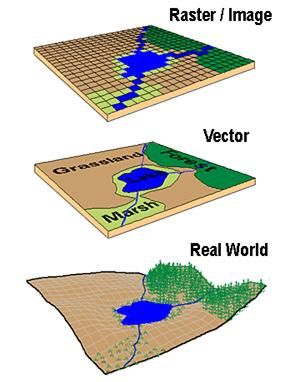
\includegraphics[width=4.16667in,height=\textheight]{general_images/rasvec.jpg}

}

\caption{Types of spatial data. Source:
\href{https://planet.uwc.ac.za/nisl/gis/web_page/page_15.htm}{Spatial
data models}}

\end{figure}

\hypertarget{projections}{%
\section{Projections}\label{projections}}

Spatial data is special as it must have a \textbf{coordinate reference
system (CRS)} often referred to as a \textbf{projection}.

These are mathematical formulas that specify how our data is represented
on a map. \textgreater{} How would you represent the globe on a 2D paper
map, screen or sphere?

Projections can either be geographic coordinate reference systems or
projected coordinate reference systems. The former treats data as a
sphere and the latter as a flat object. You might come across phrases
such as a resolution of 5 minutes or a resolution of 30 metres, which
can be used to establish what kind of projection system has been used.
Let me explain\ldots{}

A minute type of resolution (e.g.~5 minute resolution) is a geographic
reference system that treats the globe as if it was a sphere divided
into 360 equal parts called degrees (which are angular units). Each
degree has 60 minutes and each minute has 60 seconds. Arc-seconds of
latitude (horizontal lines in the globe figure below) remain almost
constant whilst arc-seconds of longitude (vertical lines in the globe
figure below) decrease in a trigonometric cosine-based fashion as you
move towards the Earth's poles.

\begin{figure}

{\centering 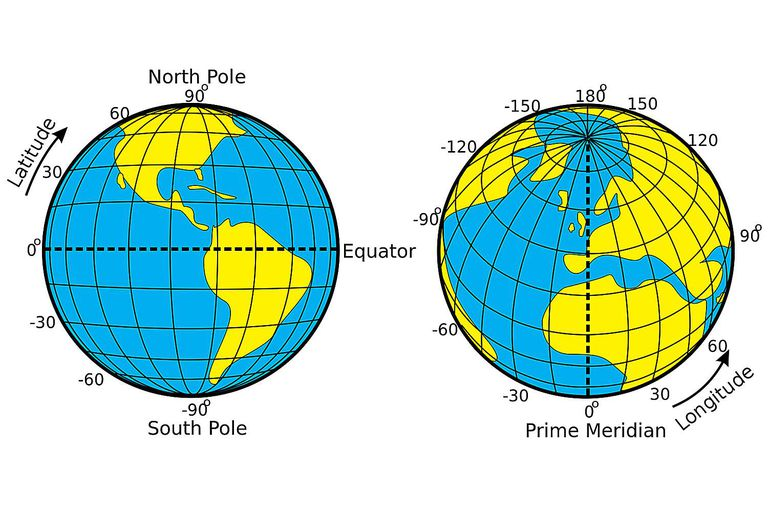
\includegraphics{prac3_images/arcseconds.jpg}

}

\caption{Latitude and Longitude. Source:
\href{https://www.thoughtco.com/degree-of-latitude-and-longitude-distance-4070616}{ThoughtCo.}}

\end{figure}

This causes problems as you increase or decrease latitude the
longitudinal lengths alter\ldots For example at the equator (0°, such as
Quito) a degree is 111.3 km whereas at 60° (such as Saint Petersburg) a
degree is 55.80 km\ldots{}

In contrast a projected coordinate system is defined on a flat,
two-dimensional plane (through projecting a spheroid onto a 2D surface)
giving it constant lengths, angles and are\ldots{}

\begin{figure}

\begin{minipage}[t]{0.50\linewidth}

{\centering 

\raisebox{-\height}{

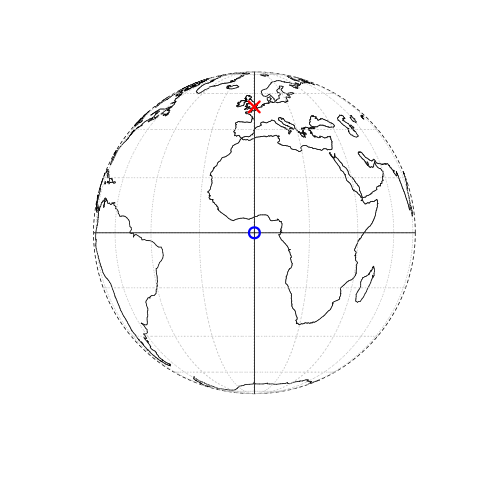
\includegraphics{general_images/vector_lonlat.png}

}

}

\end{minipage}%
%
\begin{minipage}[t]{0.50\linewidth}

{\centering 

\raisebox{-\height}{

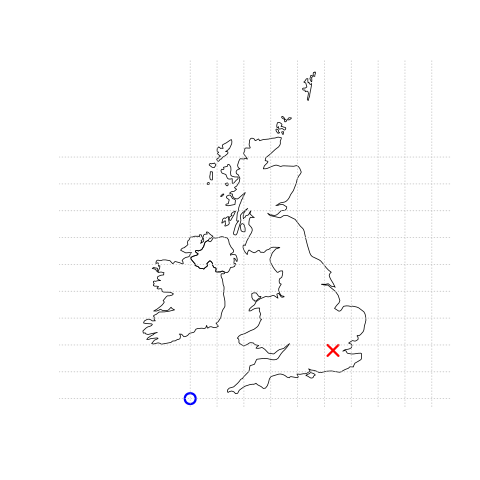
\includegraphics{general_images/vector_projected.png}

}

}

\end{minipage}%

\caption{\label{fig-elephants}Illustration of vector (point) data in
which location of London (the red X) is represented with reference to an
origin (the blue circle). The left plot (a) represents a geographic CRS
with an origin at 0° longitude and latitude. The right plot (b)
represents a projected CRS with an origin located in the sea west of the
South West Peninsula. Source:
\href{https://geocompr.robinlovelace.net/spatial-class.html}{Lovelace et
al.~(2019) section 2.2}}

\end{figure}

Knowing this, if we want to conduct analysis locally (e.g.~at a national
level) or use metric (e.g.~kilometres) measurements we need to be able
to change the projection of our data or ``reproject'' it. Most countries
and even states have their own projected coordinate reference system
such as British National Grid in the above example\ldots Note how the
origin (0,0) is has moved from the centre of the Earth to the bottom
South West corner of the UK, which has now been ironed (or flattened)
out.

\hypertarget{questions-we-can-ask}{%
\section{Questions we can ask}\label{questions-we-can-ask}}

The real benefit of spatial data is that we can see \textbf{where trends
happen}\ldots.

Examples of questions include:

\begin{itemize}
\item
  Are the pharmacies distributed randomly or do they exhibit some kind
  of dispersed or clustered pattern?
\item
  What factors influence evictions in a city (e.g.~New York)?
\item
  Are the values (e.g.~income / deprivation) similar (or dissimilar)
  across the areas of a city?
\item
  What are the factors that might lead to variation in Average GCSE
  (secondary school grades) point scores across the city?
\item
  Is there racial bias in stop question and frisk data?
\item
  What population does a hospital / school / social service cover ?
\item
  If we were to develop a new facility (e.g.~hospital, school, pharmacy)
  where would it reduce demand the most given some candidate sites ?
\item
  What factors influence perceived safety in the built envrionment?
\end{itemize}

\bookmarksetup{startatroot}

\hypertarget{getting-the-data}{%
\chapter{Getting the data}\label{getting-the-data}}

The purpose of the workshop is to:

\begin{itemize}
\tightlist
\item
  Devise a spatial question based on available data
\item
  Demonstrate how this might be achieved
\item
  The task is to explore the data, understand what it shows, see how it
  can be joined to other datasets (e.g.~raw data joined to spatial data)
  and provide some suggestions for analysis.
\end{itemize}

In the presentation we want to see:

\begin{itemize}
\tightlist
\item
  An explanation of the question, ideally with reference to local,
  national or international policy.
\item
  The data sets that will be used
\item
  Critical data reflection - What the datasets represent (and what they
  don't represent)
\item
  A methodology suggestion (note, it is not required to do any analysis)
\item
  What / who the outputs will be useful for
\end{itemize}

Data can be both spatial and non spatial. The former is some kind of
object (often a shapefile) the latter is a dataset file (such as a csv).
Typically these files will have a unique ID that we can join them on -
such as a district or ward.

\hypertarget{datasets}{%
\section{Datasets}\label{datasets}}

\begin{itemize}
\tightlist
\item
  \href{https://opencity.in/}{Open Data City}

  \begin{itemize}
  \tightlist
  \item
    Search Hyderabad
  \item
    Points for: Schools, health care facilities, parks and playgrounds,
    toilets, slums, Annapurna meals
  \item
    Polygons for: Wards
  \item
    Non spatial data: Census, Education data (number of places)
  \end{itemize}
\item
  \href{https://download.geofabrik.de/}{Open Street Map}

  \begin{itemize}
  \tightlist
  \item
    Roads
  \item
    Points of interest (e.g.~schools, tourist attractions, shops, health
    care facilities, restaurants, bakeries)
  \item
    Buildings
  \item
    Railways
  \end{itemize}
\item
  \href{https://hub.worldpop.org/project/categories?id=18}{Population
  per 1km grid cell}

  \begin{itemize}
  \tightlist
  \item
    For a variety of years
  \end{itemize}
\end{itemize}

\textbf{Census data}

I have found a variety of sources that contain census data. Some make it
difficult to join the data as there is no matching column. Last year the
\href{https://www.devdatalab.org/shrug_download/}{Development Data Lab}
complied this data for us!

You can read more about their work in
\href{https://devdatalab.medium.com/open-access-geospatial-data-for-india-b9dceb7196bb}{their
medium article}

As \textbf{village boundaries can change} between census years it is
challenging to compare values. In response they have developed a
standard zone called a \texttt{shrid} that keeps the boundaries the same
across all census years! You can decide what boundary is most
appropriate for your question - do you care about past data or is the
most recent census data sufficient?

In the 2011 village data the columns stand for:

\begin{itemize}
\tightlist
\item
  pc11\_s\_id = state
\item
  pc11\_d\_id = district
\item
  pc11\_sd\_id = sub district
\item
  pc11\_tv\_id = village
\end{itemize}

Within this site there is:

\begin{itemize}
\tightlist
\item
  Election data
\item
  Facebook population and estimated wealth
\item
  2012-2021 Night time lights (used for monitoring GPD / urban growth)
\item
  Pollution data (from satellites)
\item
  Consumption and poverty estimates
\end{itemize}

\bookmarksetup{startatroot}

\hypertarget{qgis-1}{%
\chapter{QGIS}\label{qgis-1}}

Quantum Geographical Information Systems (QGIS) is a free GIS. For the
purpose of this workshop it can assist is in \textbf{easily viewing
spatial data}. This includes point data (e.g.~csv / spreadsheet data
that has a latitude and longitude column) and spatial data such as
shapefiles, geopackages and KMLs.

From the following page you should have installed QGIS. Open the
software on your computer.

\hypertarget{data}{%
\section{Data}\label{data}}

The following data is used within this short practical.

\begin{itemize}
\tightlist
\item
  \href{https://data.opencity.in/dataset/hyderabad-schools}{Open Data
  City schools}
\item
  \href{https://download.geofabrik.de/}{Open Street Map} - points of
  interest
\item
  \href{https://hub.worldpop.org/geodata/summary?id=49804}{World pop
  population (2020)}
\item
  \href{https://www.devdatalab.org/shrug_download/}{Data Devevelopment
  Lab}

  \begin{itemize}
  \tightlist
  \item
    PC11 Subdistrict Polygons, 2011 Population Census Abstract\\
  \item
    Open Polygons and Spatial Statistics, PC11 Subdistrict Polygons
  \end{itemize}
\end{itemize}

\hypertarget{making-a-project}{%
\section{Making a project}\label{making-a-project}}

In QGIS we can make a ``project''. The project stores relatively little
information. However it will store the file path for each file you load.
Say for example we load a shapefile (like we will later), if i create
(and save) a project it will know where that file is stored and load it
next time i open the project.

To create a project: Project (top left tool bar) \textgreater{} Save as.

\hypertarget{using-qgis}{%
\section{Using QGIS}\label{using-qgis}}

\hypertarget{moving-around-the-map}{%
\subsection{Moving around the map}\label{moving-around-the-map}}

In the top tool bar there are a variety of buttons. Two are the most
used:

\begin{itemize}
\tightlist
\item
  The white hand: let's you scroll around the map
\item
  The blue i with an arrow: let's you query what value the data has.
\end{itemize}

\hypertarget{saving-data}{%
\subsection{Saving data}\label{saving-data}}

In the following sections we will be select data and exporting it.

There are many ways to export data, but two are often more common:

\begin{itemize}
\tightlist
\item
  Shapefiles - actually several files that make a shapefile
\item
  Geopackage - a container, like a folder that stores all spatial data.
  The benefit is that it is stored as a signle file meaning if we want
  to share our data we just share the 1 file!
\end{itemize}

File management is up to you.

But to make a geopacakge for this work right click on the Geopackage
name \textgreater{} create database. Select no geometry here (as the
Geopackage will not have any spatial information, but the files places
within it will)

\begin{figure}

{\centering 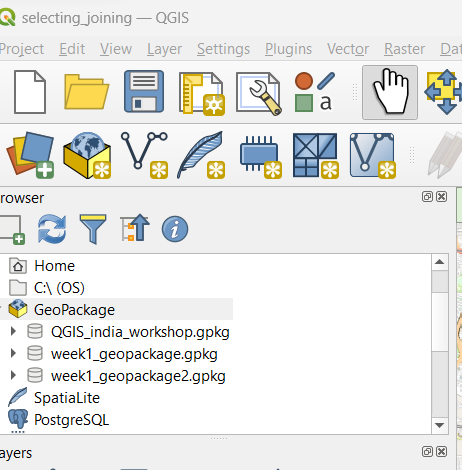
\includegraphics[width=3.73958in,height=\textheight]{general_images/geopackage.png}

}

\end{figure}

\hypertarget{adding-spatial-data}{%
\section{Adding spatial data}\label{adding-spatial-data}}

You will be presented with a blank map. To assist us in navigating on
the top tool bar select Web \textgreater{} Quick Map Services
\textgreater{} OSM \textgreater{} OSM standard

This will provide us with a ``basemap'' it is actually the same as
OpenStreetMap but the features are not queryable and it is \textbf{just
an image}.

\begin{figure}

{\centering 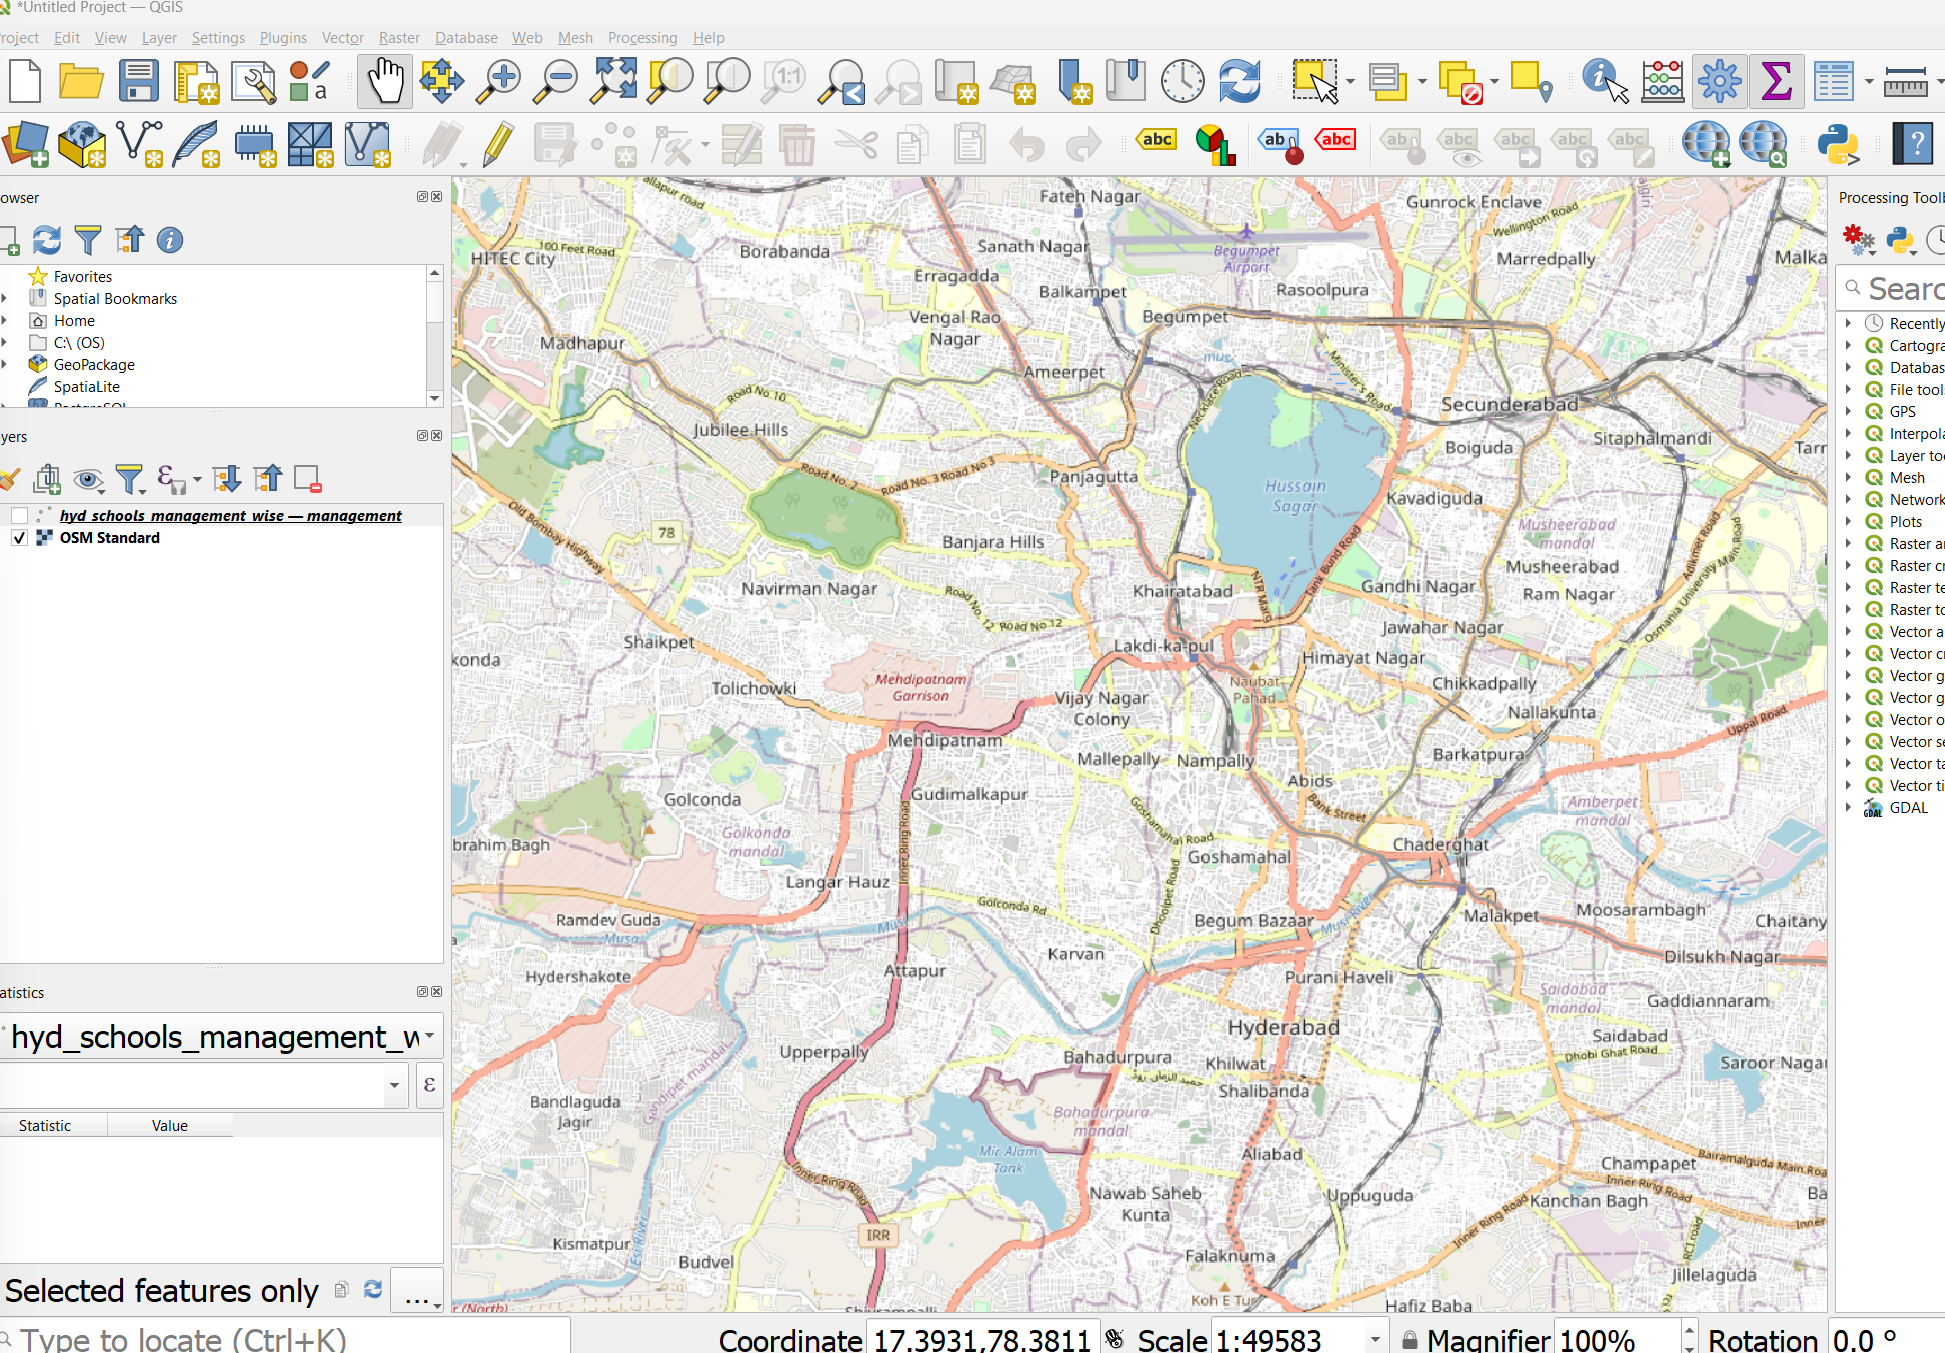
\includegraphics[width=5.61458in,height=\textheight]{general_images/basemap.png}

}

\end{figure}

Now, let's add some data. To add a spatial layer (e.g.~a shapefile) you
can simply drag and drop it into QGIS.

\textbf{Note} that a shapefile is composed of a variety of files! See
the
\href{https://andrewmaclachlan.github.io/CASA0005repo/geographic-information.html\#shapefiles}{explaination
of shapefiles}

For the purpose of this workshop select the \texttt{.shp} and drag it
in.

In a similar theme we can also drag and drop in a KML file. Here, i have
add the point of interest layer from the OpenStreetMap data (that i
downloaded) and the schools data (KML) from Open Data City. Note that we
can see the files in the \texttt{layer} tab on the left. If we uncheck a
box the layer is removed from the map.

We can also right click a layer and \texttt{zoom\ to\ layer} to see the
full extent of it (here, all the points).

\begin{figure}

{\centering 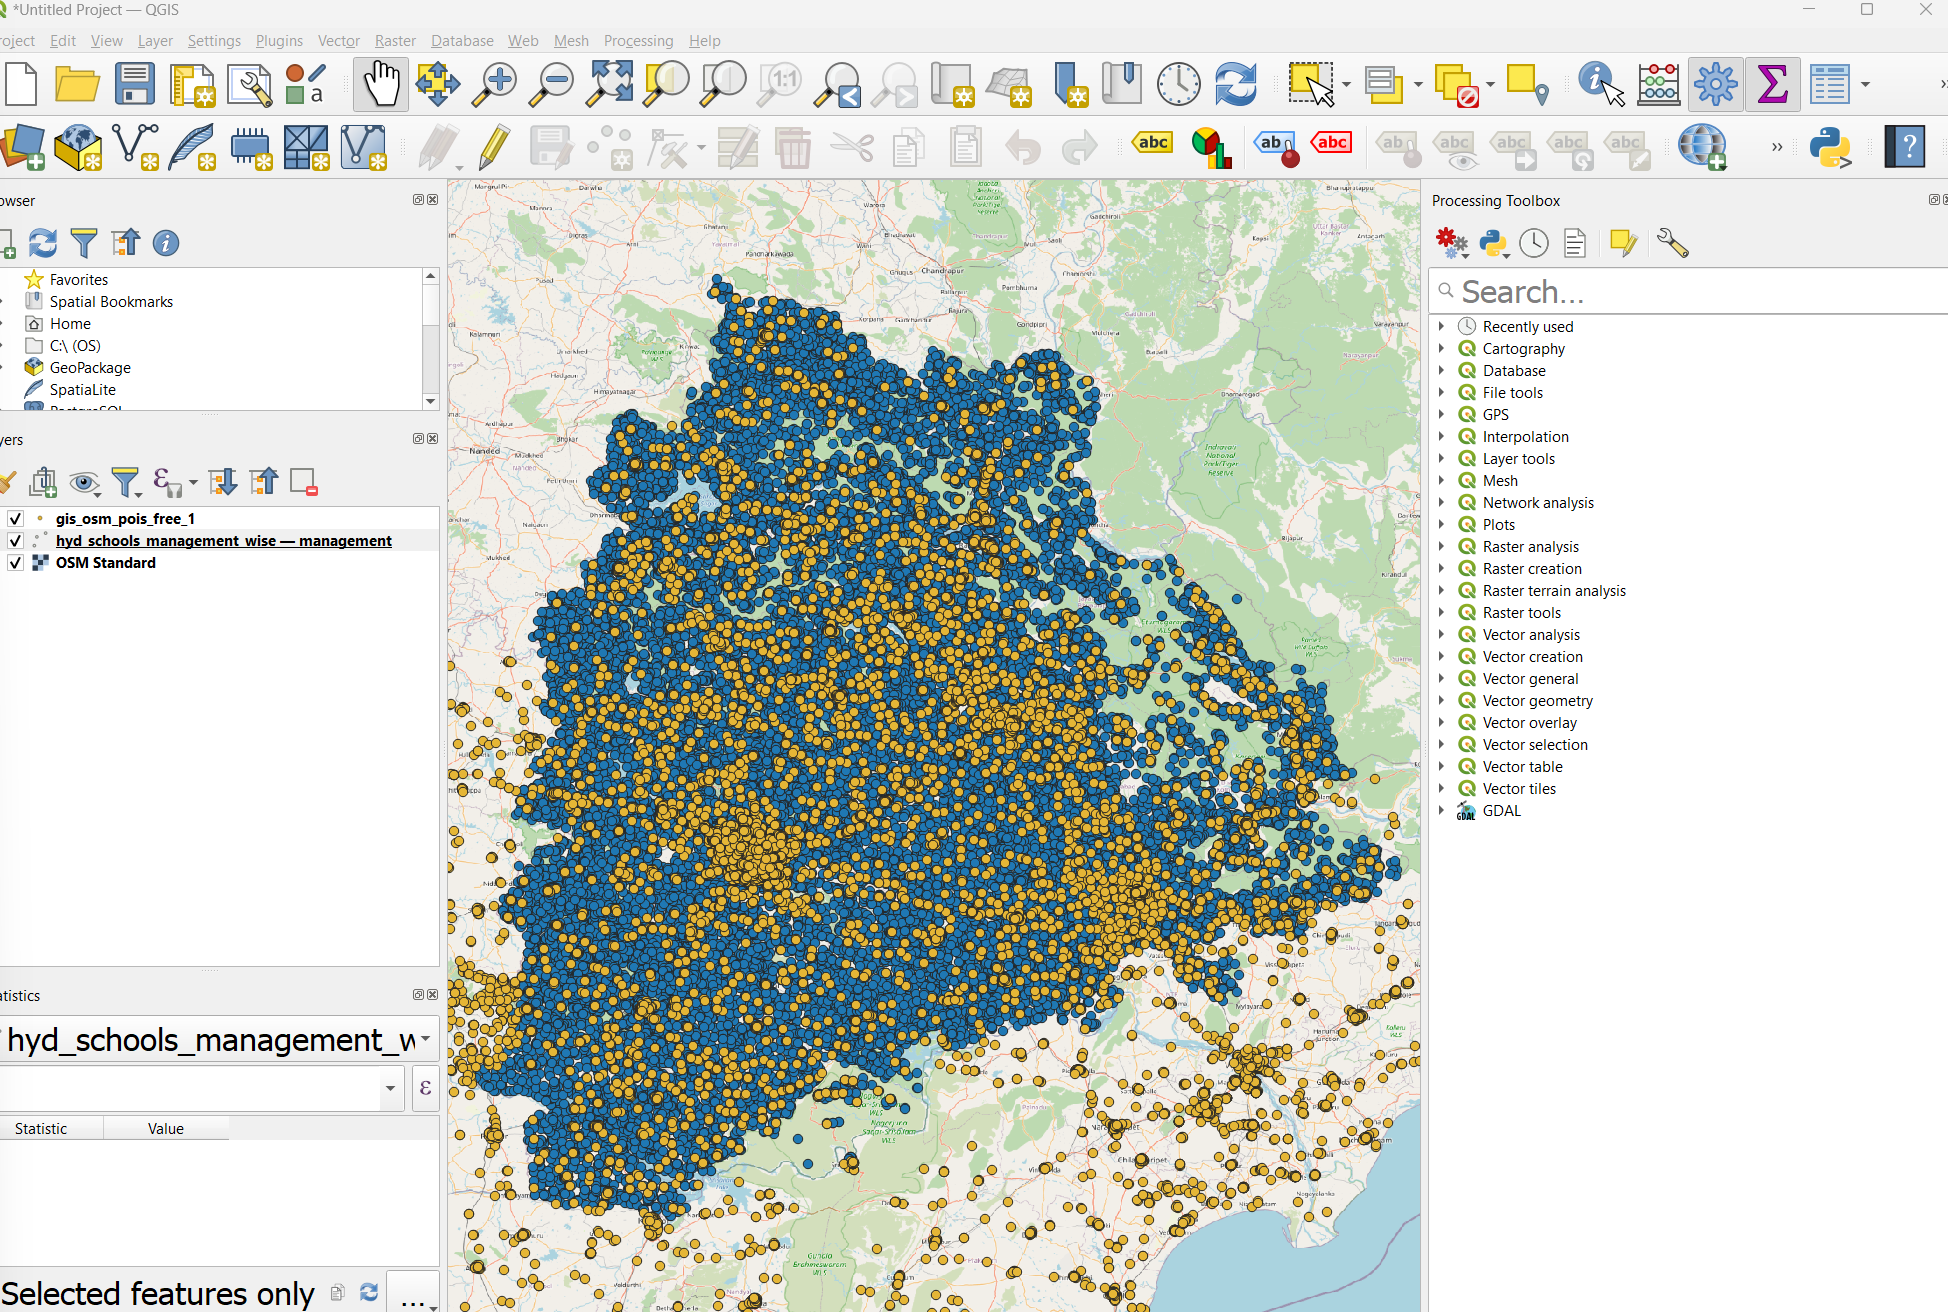
\includegraphics[width=6.0625in,height=\textheight]{general_images/all_points.png}

}

\end{figure}

\hypertarget{setting-a-cordiante-reference-system}{%
\subsection{Setting a cordiante reference
system}\label{setting-a-cordiante-reference-system}}

There are two coordinate reference systems to be aware of:

\begin{itemize}
\tightlist
\item
  That of each data layer
\item
  That of the ``map layer'' or the ``canvas'' in QGIS.
\end{itemize}

\hypertarget{crs-of-data}{%
\subsubsection{CRS of data}\label{crs-of-data}}

Each spatial layer will have a coordinate reference system. If we right
click on the point of interest layer from OSM \textgreater{} properties
\textgreater{} information. We can see that the CRS is EPSG:4326 -
WGS84.

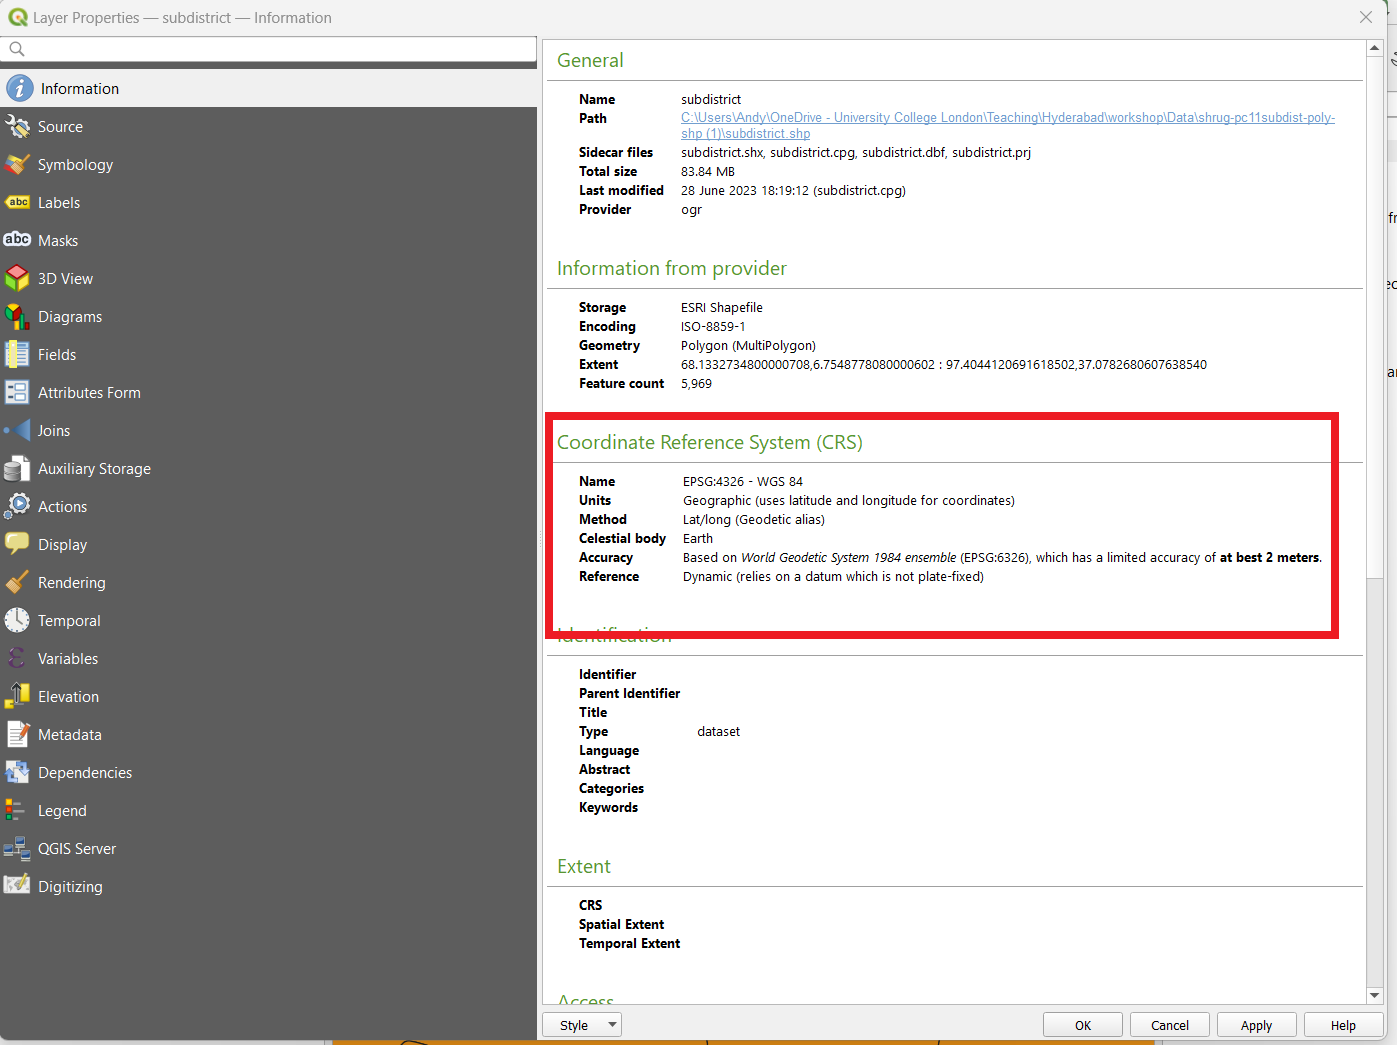
\includegraphics{general_images/properties_CRS.pdf}

If we do the same for the school data (from Open Data City) we get the
same CRS.

This is a geographic CRS and we can see that the units are in degrees -
so not very helpful if we want to work out distance!

To transform the CRS to something more use (in metric units) we can use
the \texttt{reproject\ layer} function.

First, make sure the processing toolbox is on the screen. Processing
\textgreater{} Toolbox. The processing tool should appear. Search for
Reproject layer. A good one for Hyderabad is 32644.

For this example i have transformed:

\begin{itemize}
\tightlist
\item
  The sub districts
\item
  The OSM points
\item
  The Open Data City schools
\end{itemize}

\hypertarget{crs-of-the-map}{%
\subsubsection{CRS of the map}\label{crs-of-the-map}}

In the bottom right corner of QGIS you will see an EPSG for the map -
mine is 4326. QGIS sets this \textbf{based on the first dataset loaded}.

If a new dataset is loaded that is different you will get a warning. But
QGIS \textbf{reproejcts on the fly} this means that any new data will be
shown as if it is in the map CRS.

Nevertheless we should always reproject our data before analysis to a
local CRS!

\hypertarget{adding-csv-point-data}{%
\subsection{Adding csv point data}\label{adding-csv-point-data}}

If we had a csv file with latitude and longitude as points we can add
this as a spatial layer through the
\href{https://andrewmaclachlan.github.io/CASA0005repo/geographic-information.html\#load-data}{data
source manager}.

\hypertarget{adding-raster-data}{%
\subsection{Adding raster data}\label{adding-raster-data}}

For raster data we can drag and drop it again! For example download the
\href{https://hub.worldpop.org/geodata/summary?id=49804}{worldpop 2020
estiamtes for India}

Then drag and drop!

\begin{tcolorbox}[enhanced jigsaw, toprule=.15mm, colframe=quarto-callout-tip-color-frame, coltitle=black, left=2mm, rightrule=.15mm, breakable, bottomrule=.15mm, opacityback=0, bottomtitle=1mm, title=\textcolor{quarto-callout-tip-color}{\faLightbulb}\hspace{0.5em}{Tip}, colbacktitle=quarto-callout-tip-color!10!white, titlerule=0mm, colback=white, toptitle=1mm, arc=.35mm, leftrule=.75mm, opacitybacktitle=0.6]

There are many ways we can use / extract data from a raster file. This
is beyond the workshop. But we can convert this to vector (points or
polygons) and reproject it if needed.

\end{tcolorbox}

\hypertarget{filtering}{%
\section{Filtering}\label{filtering}}

\hypertarget{by-attributes}{%
\subsection{By attributes}\label{by-attributes}}

Within my sub district data, i know that Hyderabad has a district value
of 536. However, my sub district data is for the whole if India.

To select just the sub district polygons i want. Right click on the sub
district layer in the \texttt{layers} tab (left of screen)
\textgreater{} open attribute table. At the top of the attribute table
there will be a funnel icon, click it.

You will then see all the columns of the sub district shapefile and we
can enter a filter value\ldots{}

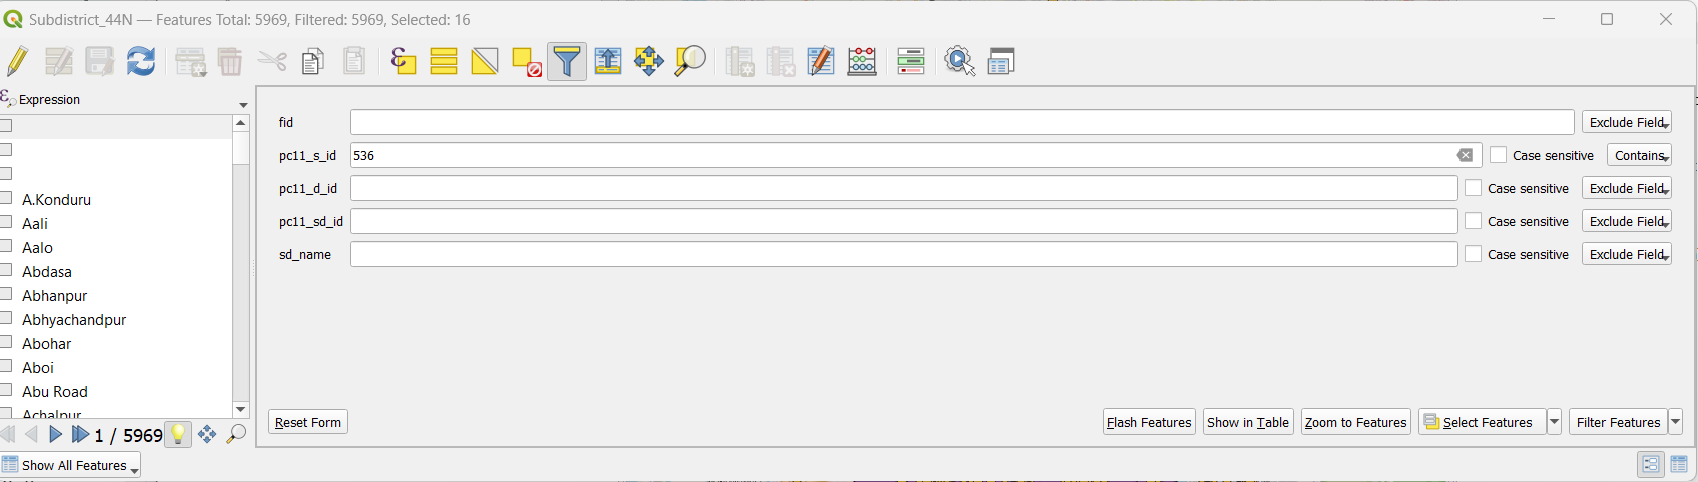
\includegraphics{general_images/filter.png}

Enter the value and click select features \textgreater{} close the
attribute table.

Go to the sub district layer \textgreater{} right click \textgreater{}
zoom to selection. You should see that the villages within Hyderabad
have been selected.

We can now export just these features. Right click the sub district
layer \textgreater{} export \textgreater{} save \textbf{selected}
features as\ldots{}

The new layer will be added to the map.

\begin{figure}

{\centering 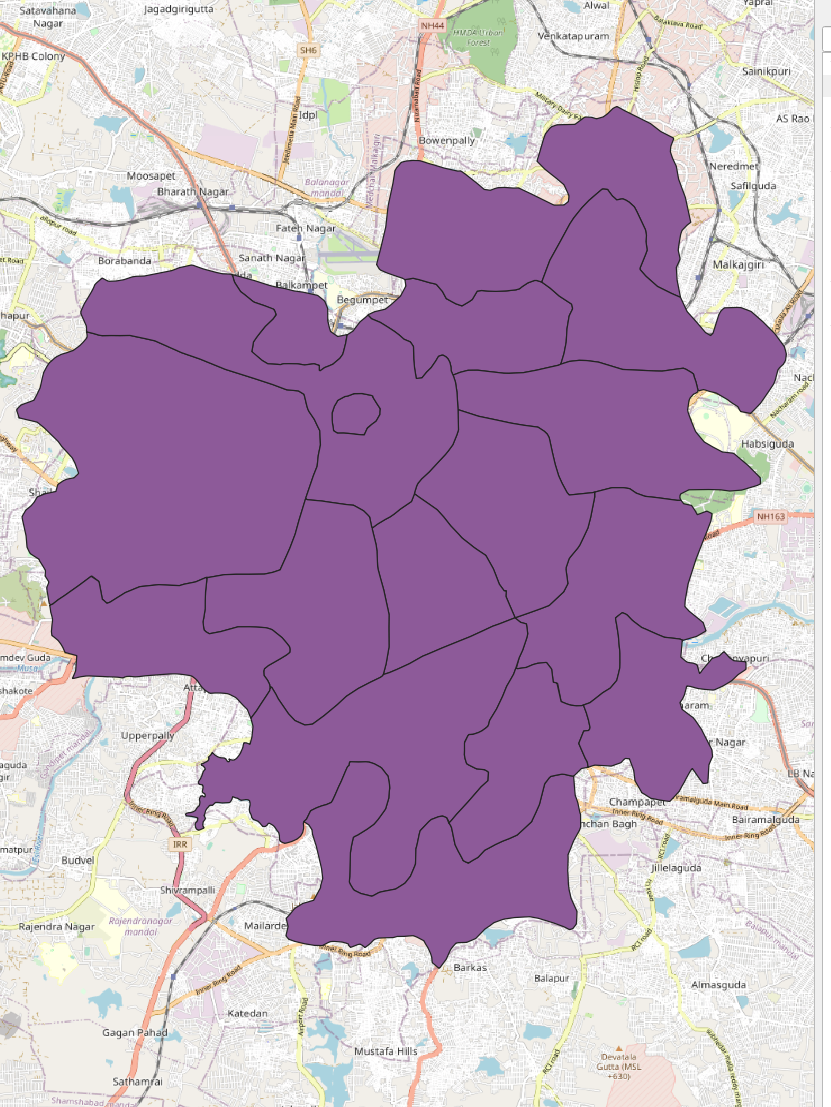
\includegraphics[width=3.08333in,height=\textheight]{general_images/Hyderabad_subdistricts.png}

}

\end{figure}

\hypertarget{by-location}{%
\subsection{By location}\label{by-location}}

If i now overlay my OpenStreetMap points of interest, it will become
quite obvious that the points go beyond our study area.

\begin{figure}

{\centering 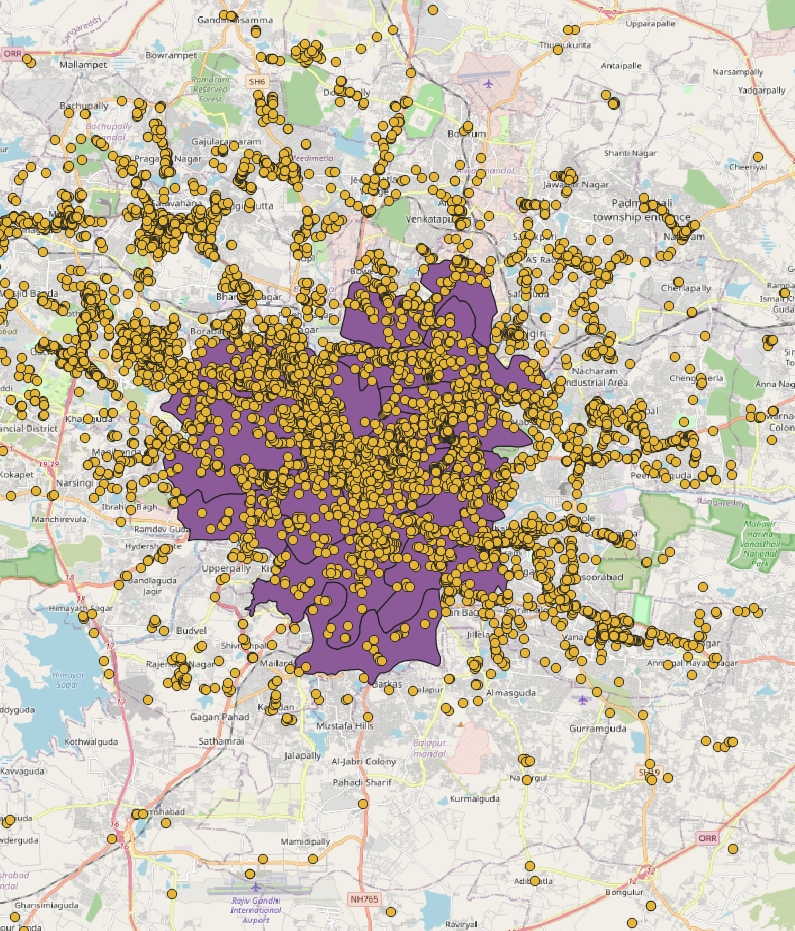
\includegraphics[width=3.85417in,height=\textheight]{general_images/points_outside_study_area.png}

}

\end{figure}

In order to constrain our points to the Hyderabad sub districts we can
select the points that intersect it, through a \textbf{select by
location}\ldots{}

Go to Vector (top toolbar) \textgreater{} research tools \textgreater{}
select by location. We want to select features \textbf{from} the points
layer (here the open street maps points) by comparing them to the
boundary of the \textbf{Hyderabad sub districts}.

You can select what \textbf{operator} to use, intersects is typically
the default in most spatial applications..

Once this has been run the points within the boundary are selected.
However, this has not been saved. If you open the attribute table of the
OpenStreetMap points in the top bar of the attribute table it will state
selected: 3488. To save our selected data we again need to right click
\textgreater{} export \textgreater{} save \textbf{selected features as}

\hypertarget{joining}{%
\section{Joining}\label{joining}}

Whilst we have completed some spatial operations we have yet to join our
census data to our spatial data.

Here, i have downloaded the
\href{https://www.devdatalab.org/shrug_download/}{2011 Population Census
Abstract data from the Development Data Lab}. This downloads as the
folder \texttt{shurg-td11-csv}. On exploring the data (in excel) i see
that it contains a sub district ID column.

Drag in the csv file from the census to QGIS layers

Right click on our Hyderabad sub districts layer \textgreater{}
properties.

On the properties window select joins (in the left column).

\begin{itemize}
\item
  Select the join layer as the csv - this is the layer to be joined to
  our spatial data
\item
  Select the join field as the sub district ID field from the csv
\item
  Select the target field as the sub district ID field from our spatial
  data:
\end{itemize}

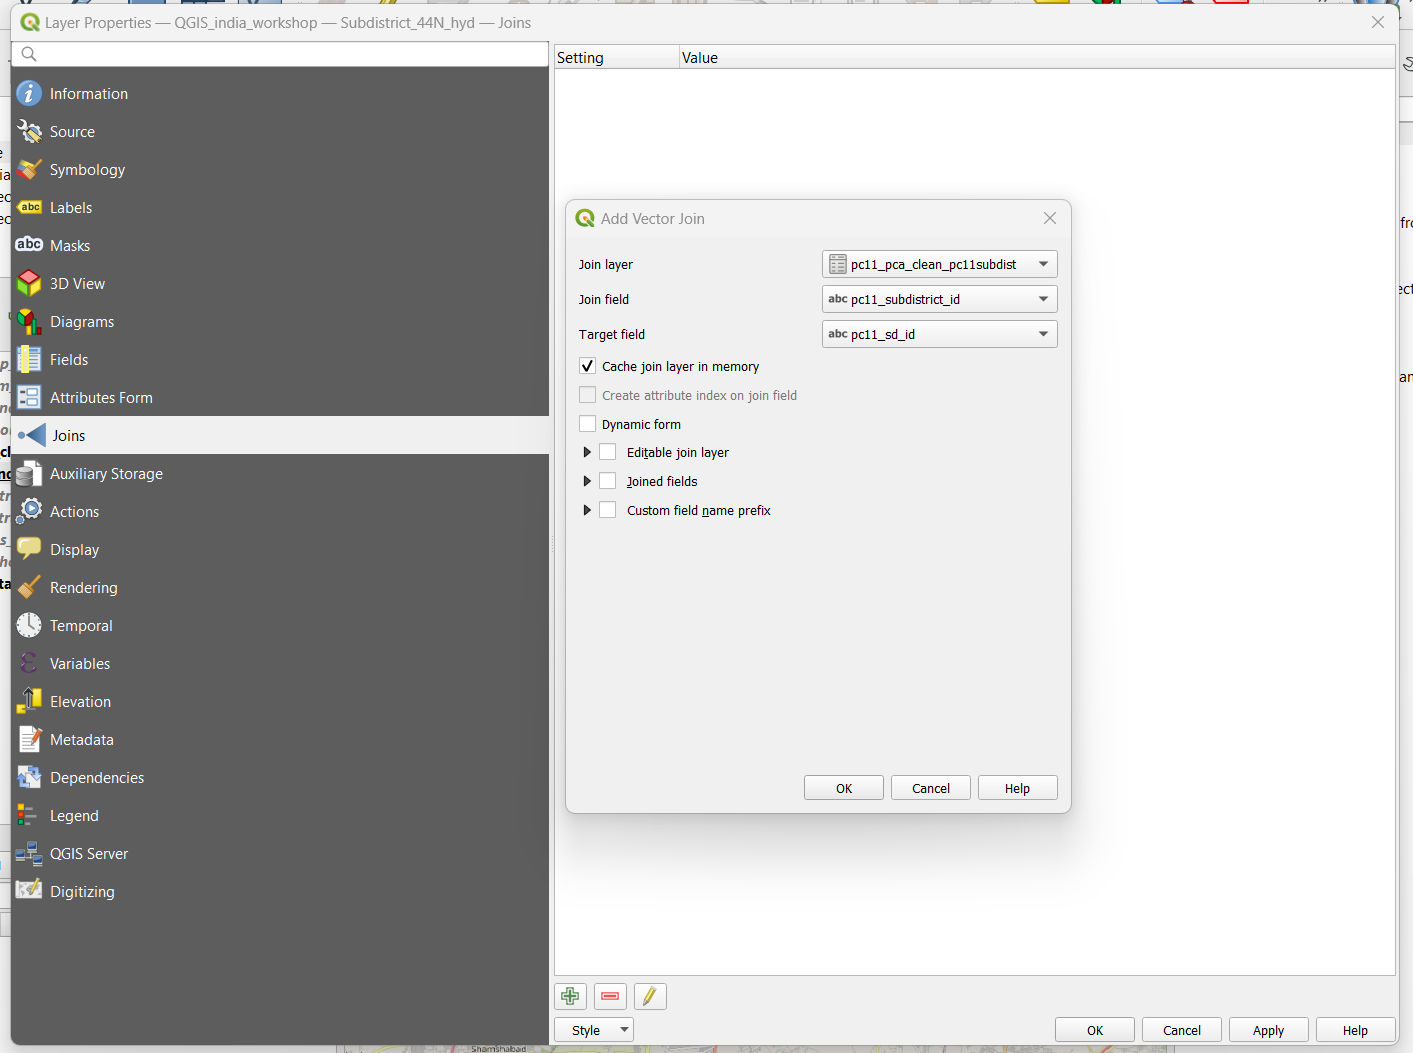
\includegraphics{general_images/joins.png}

Open the attribute table of our Hyderabad sub districts and you should
see that all the census columns are present.

\begin{tcolorbox}[enhanced jigsaw, toprule=.15mm, colframe=quarto-callout-warning-color-frame, coltitle=black, left=2mm, rightrule=.15mm, breakable, bottomrule=.15mm, opacityback=0, bottomtitle=1mm, title=\textcolor{quarto-callout-warning-color}{\faExclamationTriangle}\hspace{0.5em}{Warning}, colbacktitle=quarto-callout-warning-color!10!white, titlerule=0mm, colback=white, toptitle=1mm, arc=.35mm, leftrule=.75mm, opacitybacktitle=0.6]

\textbf{However} the join is not permanent. To keep this data you must
export the file like we have done before!

\end{tcolorbox}

\hypertarget{review}{%
\section{Review}\label{review}}

This has been a brief introduction to QGIS.

Consider the following:

\begin{itemize}
\tightlist
\item
  What is a GIS
\item
  How can we filter our data based on attrbiutes or location
\item
  How can we join non spatial data to spatial data
\end{itemize}

\bookmarksetup{startatroot}

\hypertarget{asking-questions}{%
\chapter{Asking questions}\label{asking-questions}}

Before we start asking questions of data\ldots{}

\textbf{Make a table and write down} the data you might want to use:

\begin{itemize}
\tightlist
\item
  What does it show
\item
  What does it \textbf{not show} or is missing
\item
  Does it link to spatial data
\item
  Which column links it to spatial data or does it have latitude and
  longitude (e.g.~points)
\item
  What question an we \textbf{reasonably} ask of the data
\end{itemize}

\hypertarget{questions-we-can-ask-1}{%
\section{Questions we can ask}\label{questions-we-can-ask-1}}

We need to suggest \textbf{how can we incorporate spatial data into our
question}

Given the data sets above we could seek to answer the following
questions:

\begin{itemize}
\item
  Does distance to school affect literacy outcomes

  Data:

  \begin{itemize}
  \tightlist
  \item
    Census data (literature / illiterate)
  \item
    Sub district polygons (spatial)
  \item
    School locations (coordinates provided)
  \item
    Building outlines (from open street map)
  \end{itemize}

  Analysis:

  \begin{itemize}
  \tightlist
  \item
    Make building data to points (polygons to centroids)
  \item
    Work out the average distance from each building point to each
    school per ward / district (whatever the census data is provided at)
  \item
    Plot the average distance to school against the literate column
  \end{itemize}

  Assumptions:

  \begin{itemize}
  \tightlist
  \item
    Distance might be Euclidean (as the crow flies)
  \item
    Data is from different year
  \item
    Not sure how the census assess literacy ability
  \end{itemize}
\item
  Does the location of public health services appropriately serve the
  population

  Data

  \begin{itemize}
  \tightlist
  \item
    Census data (count of people) OR
  \item
    World pop data from a more recent year
  \item
    Public health centers (point data)
  \item
    Polygon outlines (e.g.~sub districts)
  \end{itemize}

  Analysis:

  \begin{itemize}
  \tightlist
  \item
    For each word pop cell (raster cell) work out the closet public
    health centre (e.g.~direct line)
  \item
    Count the number of people assigned to each public health centre
  \item
    Compare the number of people served
  \end{itemize}

  Assumptions:

  \begin{itemize}
  \tightlist
  \item
    Different health centres might be larger or small and have more or
    less staff. How can we adjust for that? Number of staff /
    population?
  \end{itemize}
\end{itemize}

\hypertarget{your-turn}{%
\section{Your turn}\label{your-turn}}

Can you think of a similar question for:

\begin{itemize}
\tightlist
\item
  Accessing parks and playgrounds across the city
\item
  How can we estimate demand for the Annapurna food scheme locations
\end{itemize}

\bookmarksetup{startatroot}

\hypertarget{other-datasets}{%
\chapter{Other datasets}\label{other-datasets}}

\hypertarget{census}{%
\section{Census}\label{census}}

There are many websites that provide a version of census data. However,
it can be challenging to link census data (often a table) to some
spatial data (e.g.~village or districts)

Census data that i have found:

\begin{itemize}
\tightlist
\item
  \href{https://censusindia.gov.in/census.website/data/census-tables}{Indian
  census tables}

  \begin{itemize}
  \tightlist
  \item
    Note, that from my understanding Telangana was separated from Andhra
    Pradesh in 2014. This means that the census data here will probably
    not reflect current boundaries. This is not a \emph{major} issue we
    just need to ensure that it is reflected in any proposed analysis.
  \end{itemize}
\item
  \href{https://www.kaggle.com/datasets/danofer/india-census?select=india-districts-census-2011.csv}{Indian
  Census data on Kaggle}

  \begin{itemize}
  \tightlist
  \item
    This is not specific to Hyderabad
  \end{itemize}
\end{itemize}

\hypertarget{earth-observation-data}{%
\section{Earth observation data}\label{earth-observation-data}}

This is beyond the scope of the workshop but if you are interested
explore the
\href{https://developers.google.com/earth-engine/datasets}{Google Earth
Engine data catalog}


\backmatter

\end{document}
